\documentclass{standalone}


\usepackage{tikz}
\usetikzlibrary{shapes.geometric, arrows}
\usetikzlibrary{positioning}


\tikzstyle{startstop} = [rectangle, rounded corners, minimum width=2cm, minimum
height=0.5cm,text centered, draw=black]

\tikzstyle{io} = [trapezium, trapezium left angle=70, trapezium right angle=110, minimum
width=2.5cm, minimum height=0.5cm, text centered, text width = 1.5cm, draw=black]

\tikzstyle{process} = [rectangle, minimum width=2cm, minimum height=0.5cm, text centered,
text width = 1cm, draw=black]
\tikzstyle{decision} = [diamond, minimum width=2cm, minimum height=0.5cm, text centered,
draw=black]

\tikzstyle{block1} = [rectangle, rounded corners, minimum width=0.5cm, minimum
height=0.25cm,text centered, draw=black]

\tikzstyle{block2} = [rectangle, rounded corners, minimum width=2.5cm, minimum
height=3.6cm,text centered, draw=black]



\tikzstyle{arrow} = [thick,->,>=stealth]


\usetikzlibrary{calc}
\begin{document}

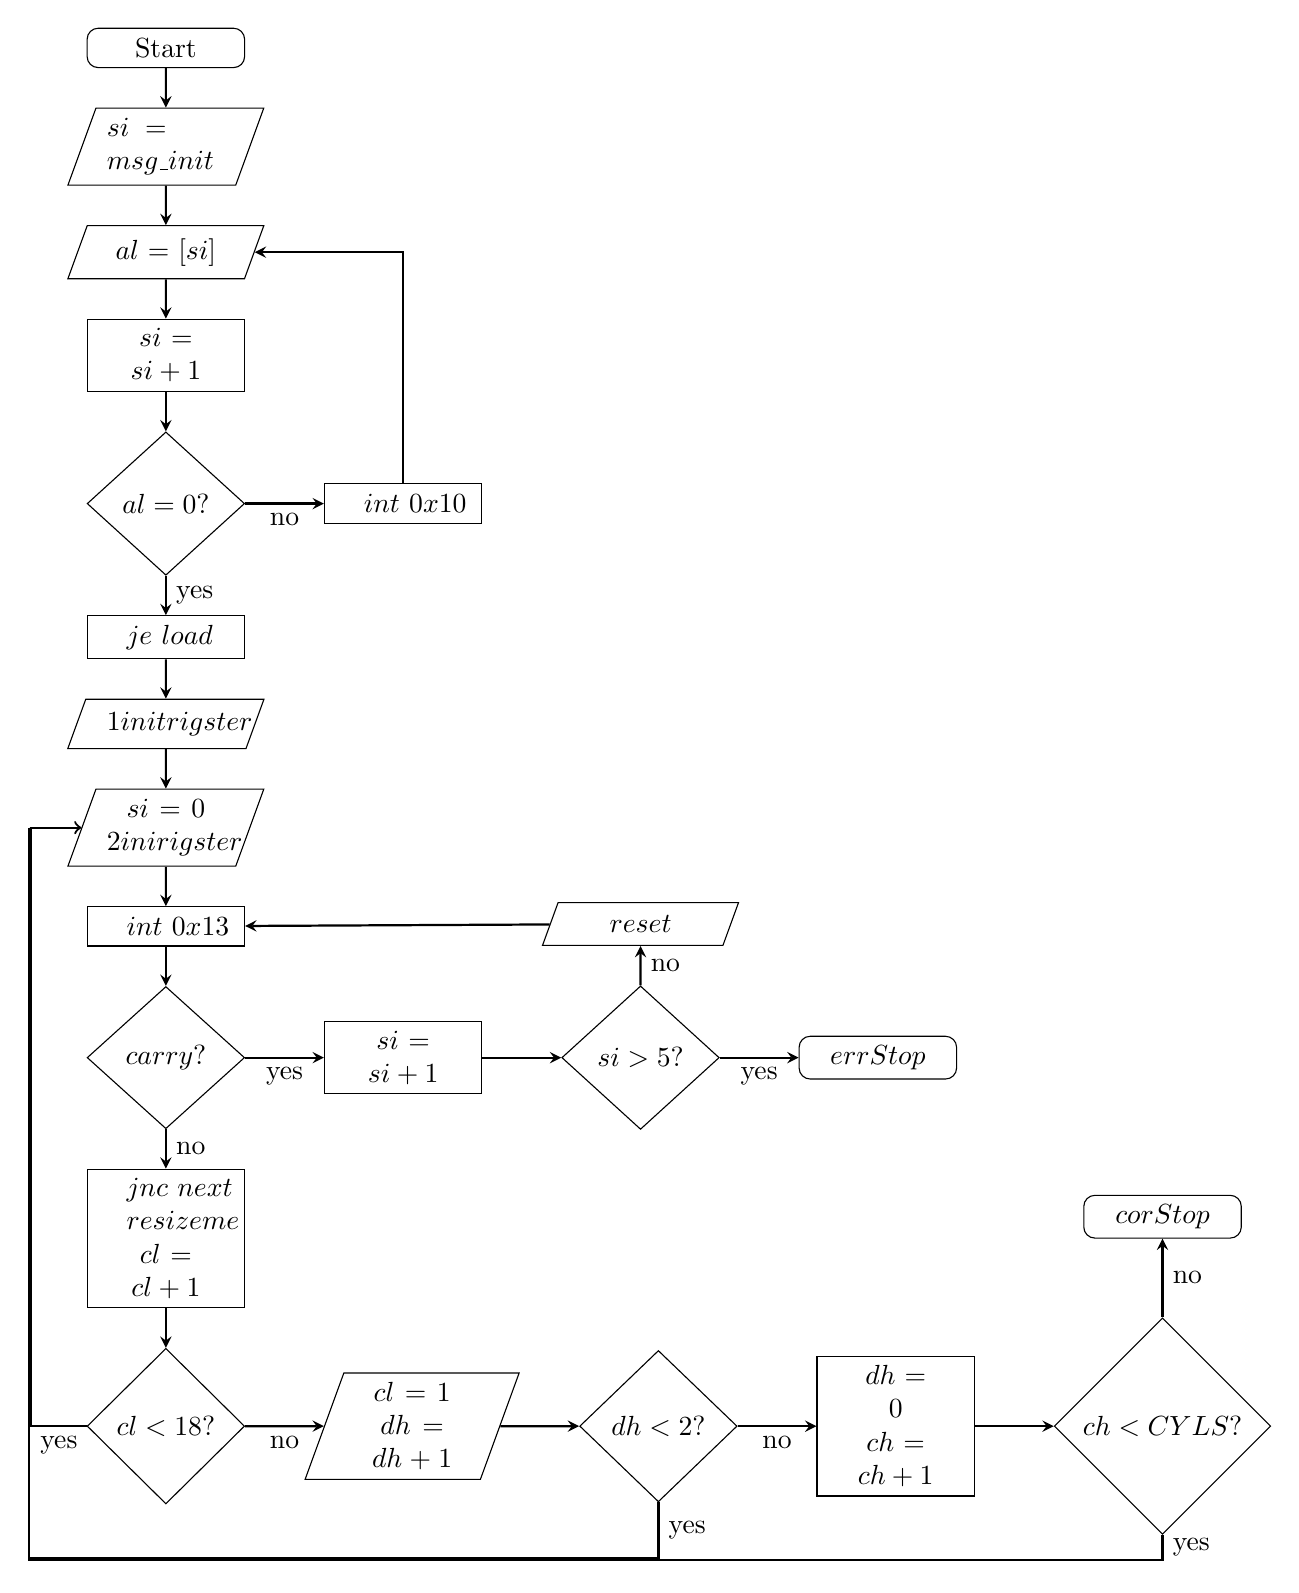
\begin{tikzpicture} [node distance=1cm]
    \node (start) [startstop, yshift=0.5cm]  {Start};
    \node (in1) [io, below=of start,align=left, yshift=0.5cm]{$si=msg\_init$};
    \node (in2) [io, below=of in1, align=center, yshift=0.5cm, align=center]{$al=[si]$};
    \node (pro1) [process, below=of in2, yshift=0.5cm] {$si=si+1$};
    \node (dec1) [decision, below=of pro1, yshift=0.5cm] {$al=0?$};
    \node (pro2) [process, right=of dec1] {$int\ 0x10$};
    \node (pro3) [process, below=of dec1, yshift=0.5cm] {$je\ load$};
    \node (in3) [io, below=of pro3, yshift=0.5cm] {$1initrigster$};
    \node (in4) [io, below=of in3, yshift=0.5cm, align=center] {$si=0$\\$2inirigster$};
    \node (pro4) [process, below=of in4, yshift=0.5cm] {$int\ 0x13$};
    \node (dec2) [decision, below=of pro4, yshift=0.5cm] {$carry?$};
    \node (pro5) [process, right=of dec2] {$si=si+1$};
    \node (dec3) [decision, right=of pro5] {$si>5?$};
    \node (in6) [io, above=of dec3, align=center, yshift=-0.5cm] {$reset$};
    \node (stop1) [startstop, right=of dec3] {$errStop$};
    \node (pro7) [process, below=of dec2, yshift=0.5cm] {$jnc\ next$\\$resizeme$\\$cl=cl+1$};
    \node (dec4) [decision, below=of pro7, yshift=0.5cm] {$cl<18?$};
    \node (in7) [io, right=of dec4] {$cl=1$\\$dh=dh+1$};
    \node (dec5) [decision, right=of in7] {$dh<2?$};
    \node (pro8) [process, right=of dec5] {$dh=0$\\$ch=ch+1$};
    \node (dec6) [decision, right=of pro8] {$ch<CYLS?$};
    \node (stop2) [startstop, above=of dec6] {$corStop$};

    \draw[-, thick] (in4.west) ($(in4.west) + (-1.9em, 0)$)|- ($(dec6.south) + (0,
    -0.9em)$) to node [auto, swap] {yes} (dec6.south);
    
    \draw[-, thick] (in4.west) ($(in4.west) + (-1.9em, 0)$)|- ($(dec5.south) + (0, -2em)$) to node [auto, swap] {yes} (dec5.south);
    \draw[<-, thick] (in4.west) -| ($(dec4.west) + (-2em,0)$) to node [auto, swap] {yes}
    (dec4.west);
    \draw[arrow] (dec6) -- node[anchor=west] {no} (stop2);
    \draw[arrow] (pro8) -- (dec6);
    \draw[arrow] (dec5) --node[anchor=north] {no} (pro8);
    \draw[arrow] (in7) -- (dec5);
    \draw[arrow] (dec4) -- node[anchor=north] {no} (in7);
    \draw[arrow] (pro7) -- (dec4);
    \draw[arrow] (dec2) -- node[anchor=west] {no} (pro7);
    \draw[arrow] (dec3) -- node[anchor=north] {yes} (stop1);
    \draw[arrow] (in6) -- (pro4);
    \draw[arrow] (dec3) -- node[anchor=west] {no} (in6);
    \draw[arrow] (pro5) -- (dec3);
    \draw[arrow] (dec2) -- node[anchor=north] {yes} (pro5);
    \draw[arrow] (pro4) -- (dec2);
    \draw[arrow] (in4) -- (pro4);
    \draw[arrow] (in3) -- (in4);
    \draw[arrow] (pro3) -- (in3);
    \draw[arrow] (dec1) -- node[anchor=west] {yes} (pro3);
    \draw[arrow] (pro2) |- (in2);
    \draw[arrow] (dec1) -- node[anchor=north] {no} (pro2);
    \draw[arrow] (start) -- (in1);
    \draw[arrow] (in1) -- (in2);
    \draw[arrow] (in2) -- (pro1);
    \draw[arrow] (pro1) -- (dec1);
    
\end{tikzpicture}
\end{document}

%%% Local Variables:
%%% mode: latex
%%% TeX-master: t
%%% End:
